% Project Specifications

\chapter{Implementation Details}

\section{Development Environment and Method}

Xilinx Vivado version 2017.04 is used as the development platform for FPGA. The typical workflow involves
the following steps: design the functionality of module, implement the module in Verilog, add IP blocks
if necessary, write the testbench for the module, run behavioral simulation, run synthesis and implementation,
run post-synthesis and post-implementation simulation, view synthesis and implementation reports, and finally,
create bitstream and test on device.

A parallel C implementation is developed on Linux simultaneously to facilitate the FPGA development.
Its main function is to provide algorithm verification, especially numerical comparison of output layers
between software implementation and FPGA implementation.

\section{Implementing the Transposed Convolutional Layer}

The DSP48 Macro IP is utilized to accomplish computations with multiplication and accumulation. The first
block implements the operations shown in \ref{table:dsp48_0_operations}. The second block is the core MACC
unit, and only contains $P \leftarrow A*B+P$.

\begin{table}[h]
  \centering
  \caption{DSP48 0 Operations}
  \begin{tabular}{l | l}
    0 & $P \leftarrow A*B-C$ \\
    1 & $P \leftarrow A*B+PCIN$ \\
    2 & $P \leftarrow A*B+C$
  \end{tabular}
  \label{table:dsp48_0_operations}
\end{table}

The ports of both blocks are shown in \ref{fig:dsp48_macro_0} and \ref{fig:dsp48_macro_1}.

\begin{figure}[h]
  \centering
  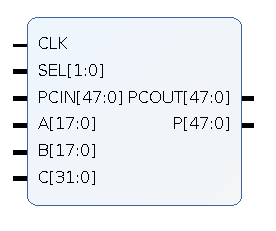
\includegraphics[scale=0.5]{dsp48_macro_0}
  \caption{DSP48 Macro 0 Ports}
  \label{fig:dsp48_macro_0}
\end{figure}

\begin{figure}[h]
  \centering
  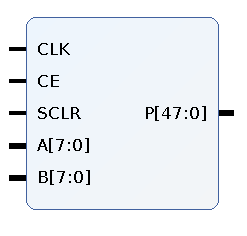
\includegraphics[scale=0.5]{dsp48_macro_1}
  \caption{DSP48 Macro 1 (MACC) Ports}
  \label{fig:dsp48_macro_1}
\end{figure}

\subsection{DSP48 Pipelining}

The DSP48 slice can be used without pipelining. However, that is essentially a combinational circuit and
the propagation delay will significantly reduce $F_{max}$. To run the FPGA at a higher frequency, it is
necessary to use pipeline registers. In our first design, only the register after the multiplier is used
therefore the result is delayed by one clock cycle.

\begin{figure}[h]
  \centering
  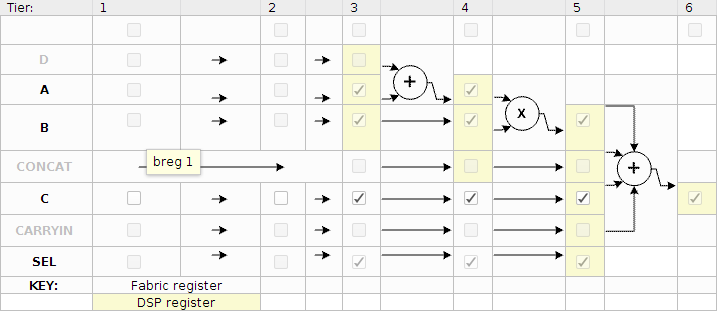
\includegraphics[scale=0.5]{dsp48_macro_0_pipeline}
  \caption{DSP48 Macro 0 Pipeline Configuration}
  \label{fig:dsp48_macro_0_pipeline}
\end{figure}

\clearpage %force the next chapter to start on a new page. Keep that as the last line of your chapter!
